%---------------------------------------------------------------------------
%	PACKAGES AND OTHER DOCUMENT CONFIGURATIONS
%---------------------------------------------------------------------------
\documentclass[final]{beamer}
\usepackage{gensymb}
\usepackage{textcomp}
\usepackage[scale=1.24]{beamerposter} % Use the beamerposter package for laying out the poster
\usetheme{confposter} % Use the confposter theme supplied with this template
\setbeamercolor{block title}{fg=Maroon,bg=white} % Colors of the block titles
\setbeamercolor{block body}{fg=black,bg=white} % Colors of the body of blocks
\setbeamercolor{block alerted title}{fg=white,bg=Maroon} % Colors of the highlighted block titles
\setbeamercolor{block alerted body}{fg=black,bg=Goldenrod!15} % Colors of the body of highlighted blocks
% Many more colors are available for use in beamerthemeconfposter.sty
%---------------------------------------------------------------------------
% Define the column widths and overall poster size
% To set effective sepwid, onecolwid and twocolwid values, first choose how many columns you want and how much separation you want between columns
% In this template, the separation width chosen is 0.024 of the paper width and a 4-column layout
% onecolwid should therefore be (1-(# of columns+1)*sepwid)/# of columns e.g. (1-(4+1)*0.024)/4 = 0.22
% Set twocolwid to be (2*onecolwid)+sepwid = 0.464
% Set threecolwid to be (3*onecolwid)+2*sepwid = 0.708
\newlength{\sepwid}
\newlength{\onecolwid}
\newlength{\twocolwid}
\newlength{\threecolwid}
\setlength{\paperwidth}{48in} % A0 width: 46.8in
\setlength{\paperheight}{38.4in} % A0 height: 33.1in
\setlength{\sepwid}{0.024\paperwidth} % Separation width (white space) between columns
\setlength{\onecolwid}{0.22\paperwidth} % Width of one column
\setlength{\twocolwid}{0.464\paperwidth} % Width of two columns
\setlength{\threecolwid}{0.708\paperwidth} % Width of three columns
\setlength{\topmargin}{-0.75in} % Reduce the top margin size
%---------------------------------------------------------------------------
\usepackage{graphicx}  % Required for including images
\usepackage{booktabs} % Top and bottom rules for tables
%---------------------------------------------------------------------------
%	TITLE SECTION 
%---------------------------------------------------------------------------
\title{Heritability of subcortical volumes \\ in the adolescent brain} % Poster title
\author{Christian Coffman Advised by: Dr. Saonli Basu and Dr. Eric Feczko} % Author(s)
\institute{Division of Biostatistics, University of Minnesota} % Institution(s)
%----------------------------------------------------------------------------

\begin{document}
\addtobeamertemplate{headline}{} 
{\begin{tikzpicture}[remember picture,overlay] 
\node [shift={(-18cm,-9cm)}] at (current page.north east) {
\includegraphics[height=10cm]{Graphics/umn-logo.png}}; 
\end{tikzpicture}
\begin{tikzpicture}[remember picture,overlay] 
\node [shift={(-105cm,-9cm)}] at (current page.north east) {
\includegraphics[height=5cm]{Graphics/sph_logo.png}}; 
\end{tikzpicture}
}
\begin{frame}[t] % The whole poster is enclosed in one beamer frame
\begin{columns}[t] % The whole poster consists of three major columns, the second of which is split into two columns twice - the [t] option aligns each column's content to the top
\begin{column}{\sepwid}\end{column} % Empty spacer column
\begin{column}{\onecolwid} % The first column
%----------------------------------------------------------------------------
%	LEFT
%---------------------------------------------------------------------------
\begin{block}{Introduction and Objectives}
Clinically diagonosoed psychological disorders are associated with heritable regional subcortical brain volumes (rSBVs) in adults \cite{koolschijn_brain_2009, zhao_heritability_2019}. To see if the same regions are heritable in adolescents, we analyzed rSBVs in the Adolescent Brain Cognitive Development study (ABCD) whih has 10,000+ structrural fMRI scans. Estimating Imaging derived phenotypes taken across multiple sites is complicated by confounding differences between sites \cite{bayer_site_2022}. In addition, sites have different distributions of subjects with respect to their genetic ancestries. Currently, no method of moments (MOM) estimator accounts for both influences which is important to get unbiased estimates.
\end{block}


\begin{block}{Methods}
\begin{enumerate}
    \item AdjHE is closed form solution to 2nd moment \cite{lin_estimating_2022}
    \item Compared to existing methods for site effects theoretically and via simulations see (Figure \ref{fig:03-03})
    \item Estimated on rSBV's in ABCD (see Figure \ref{fig:brain})
\end{enumerate}

\end{block}

\begin{block}{Estimation Time}
	\begin{figure}
		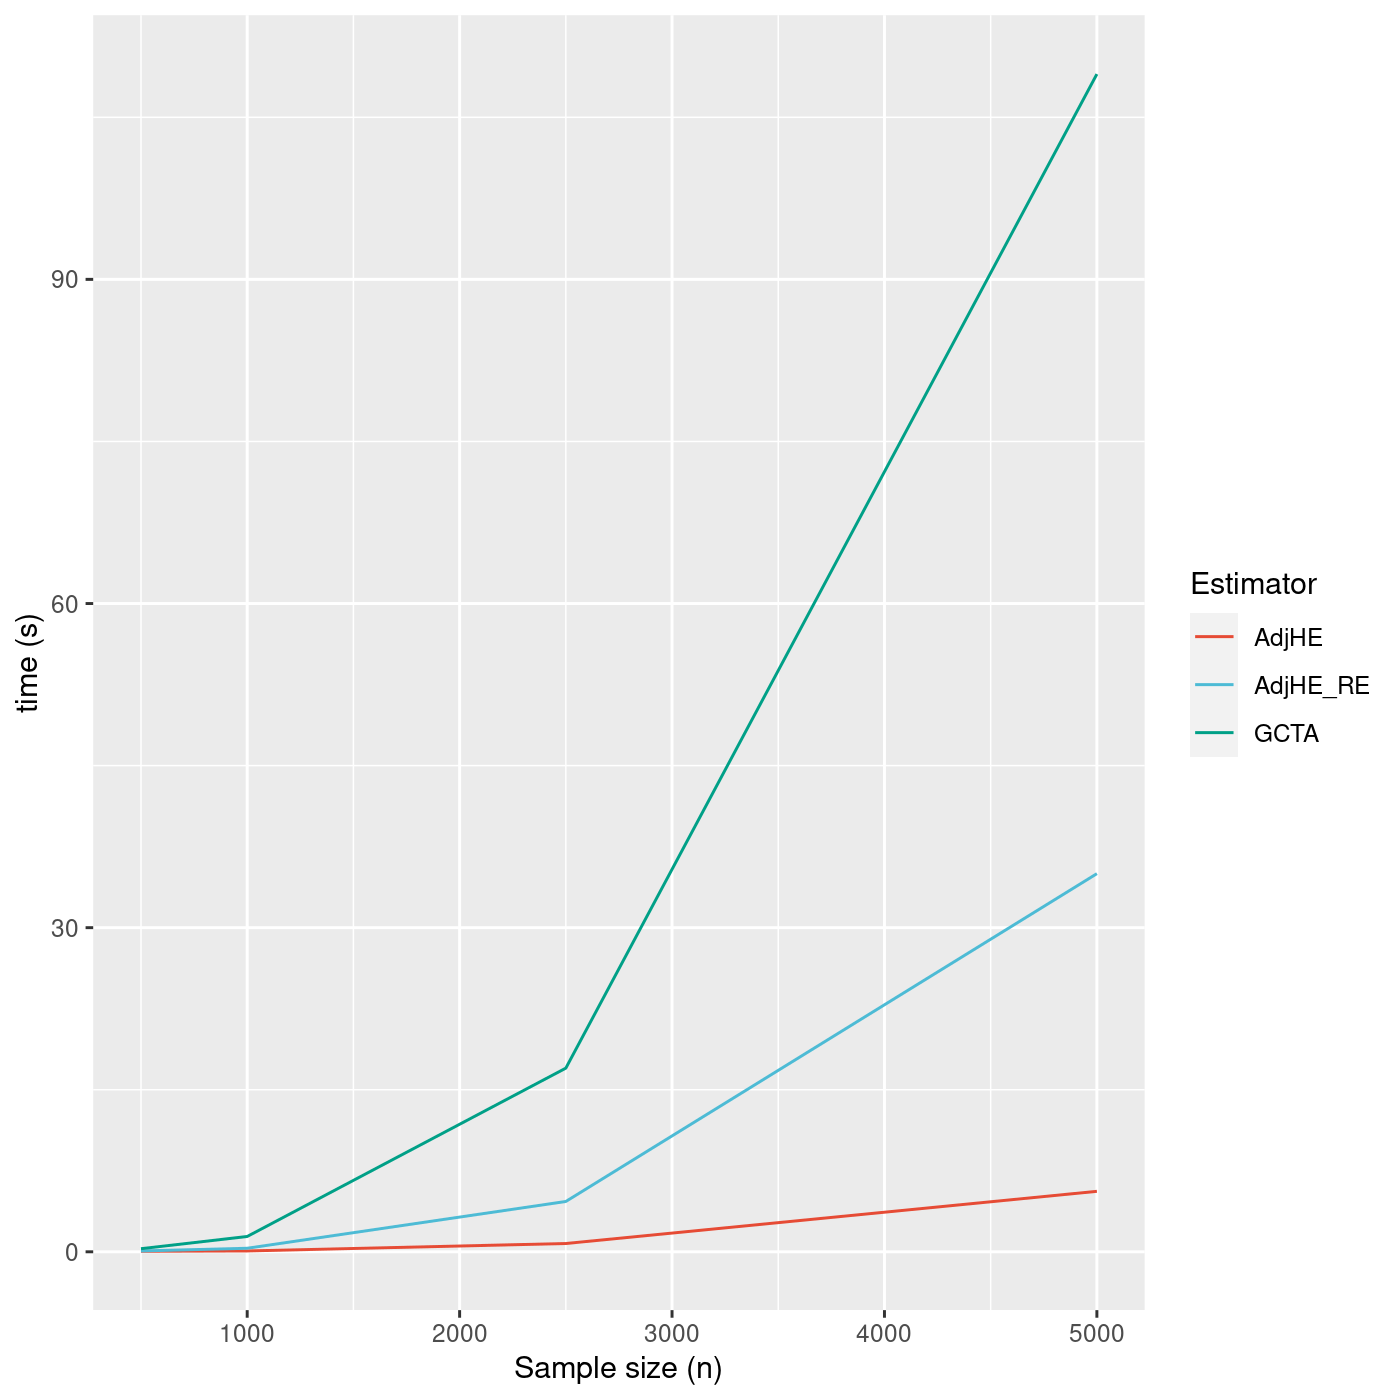
\includegraphics[width=\textwidth]{Graphics/compare_time.png}
		\caption{\centering
			Time for estimation on increasinly large simulated datsets for AdjHE (blue), AdjHE with random site effects (light blue), and GCTA (red)	
		}
	\end{figure}
\end{block}

\vspace{1in}


\end{column} % End of the first column
\begin{column}{\sepwid}\end{column} % Empty spacer column
\begin{column}{\twocolwid} % Begin a column which is two columns wide (column 2)
%----------------------------------------------------------------------------
%        MIDDLE
%----------------------------------------------------------------------------
\begin{alertblock}{rSBV Heritability}
\begin{figure}
\includegraphics[width = 1\textwidth]{Graphics/AdjHE_RE_brain.png}
\caption{Heritability of rSBVs visualized on the Conte brain template. Yellow indicates high heritability, red indicates low.}
\label{fig:brain}
\end{figure}
\end{alertblock}
%----------------------------------------------------------------------------
\vspace{2cm}
\begin{figure}
    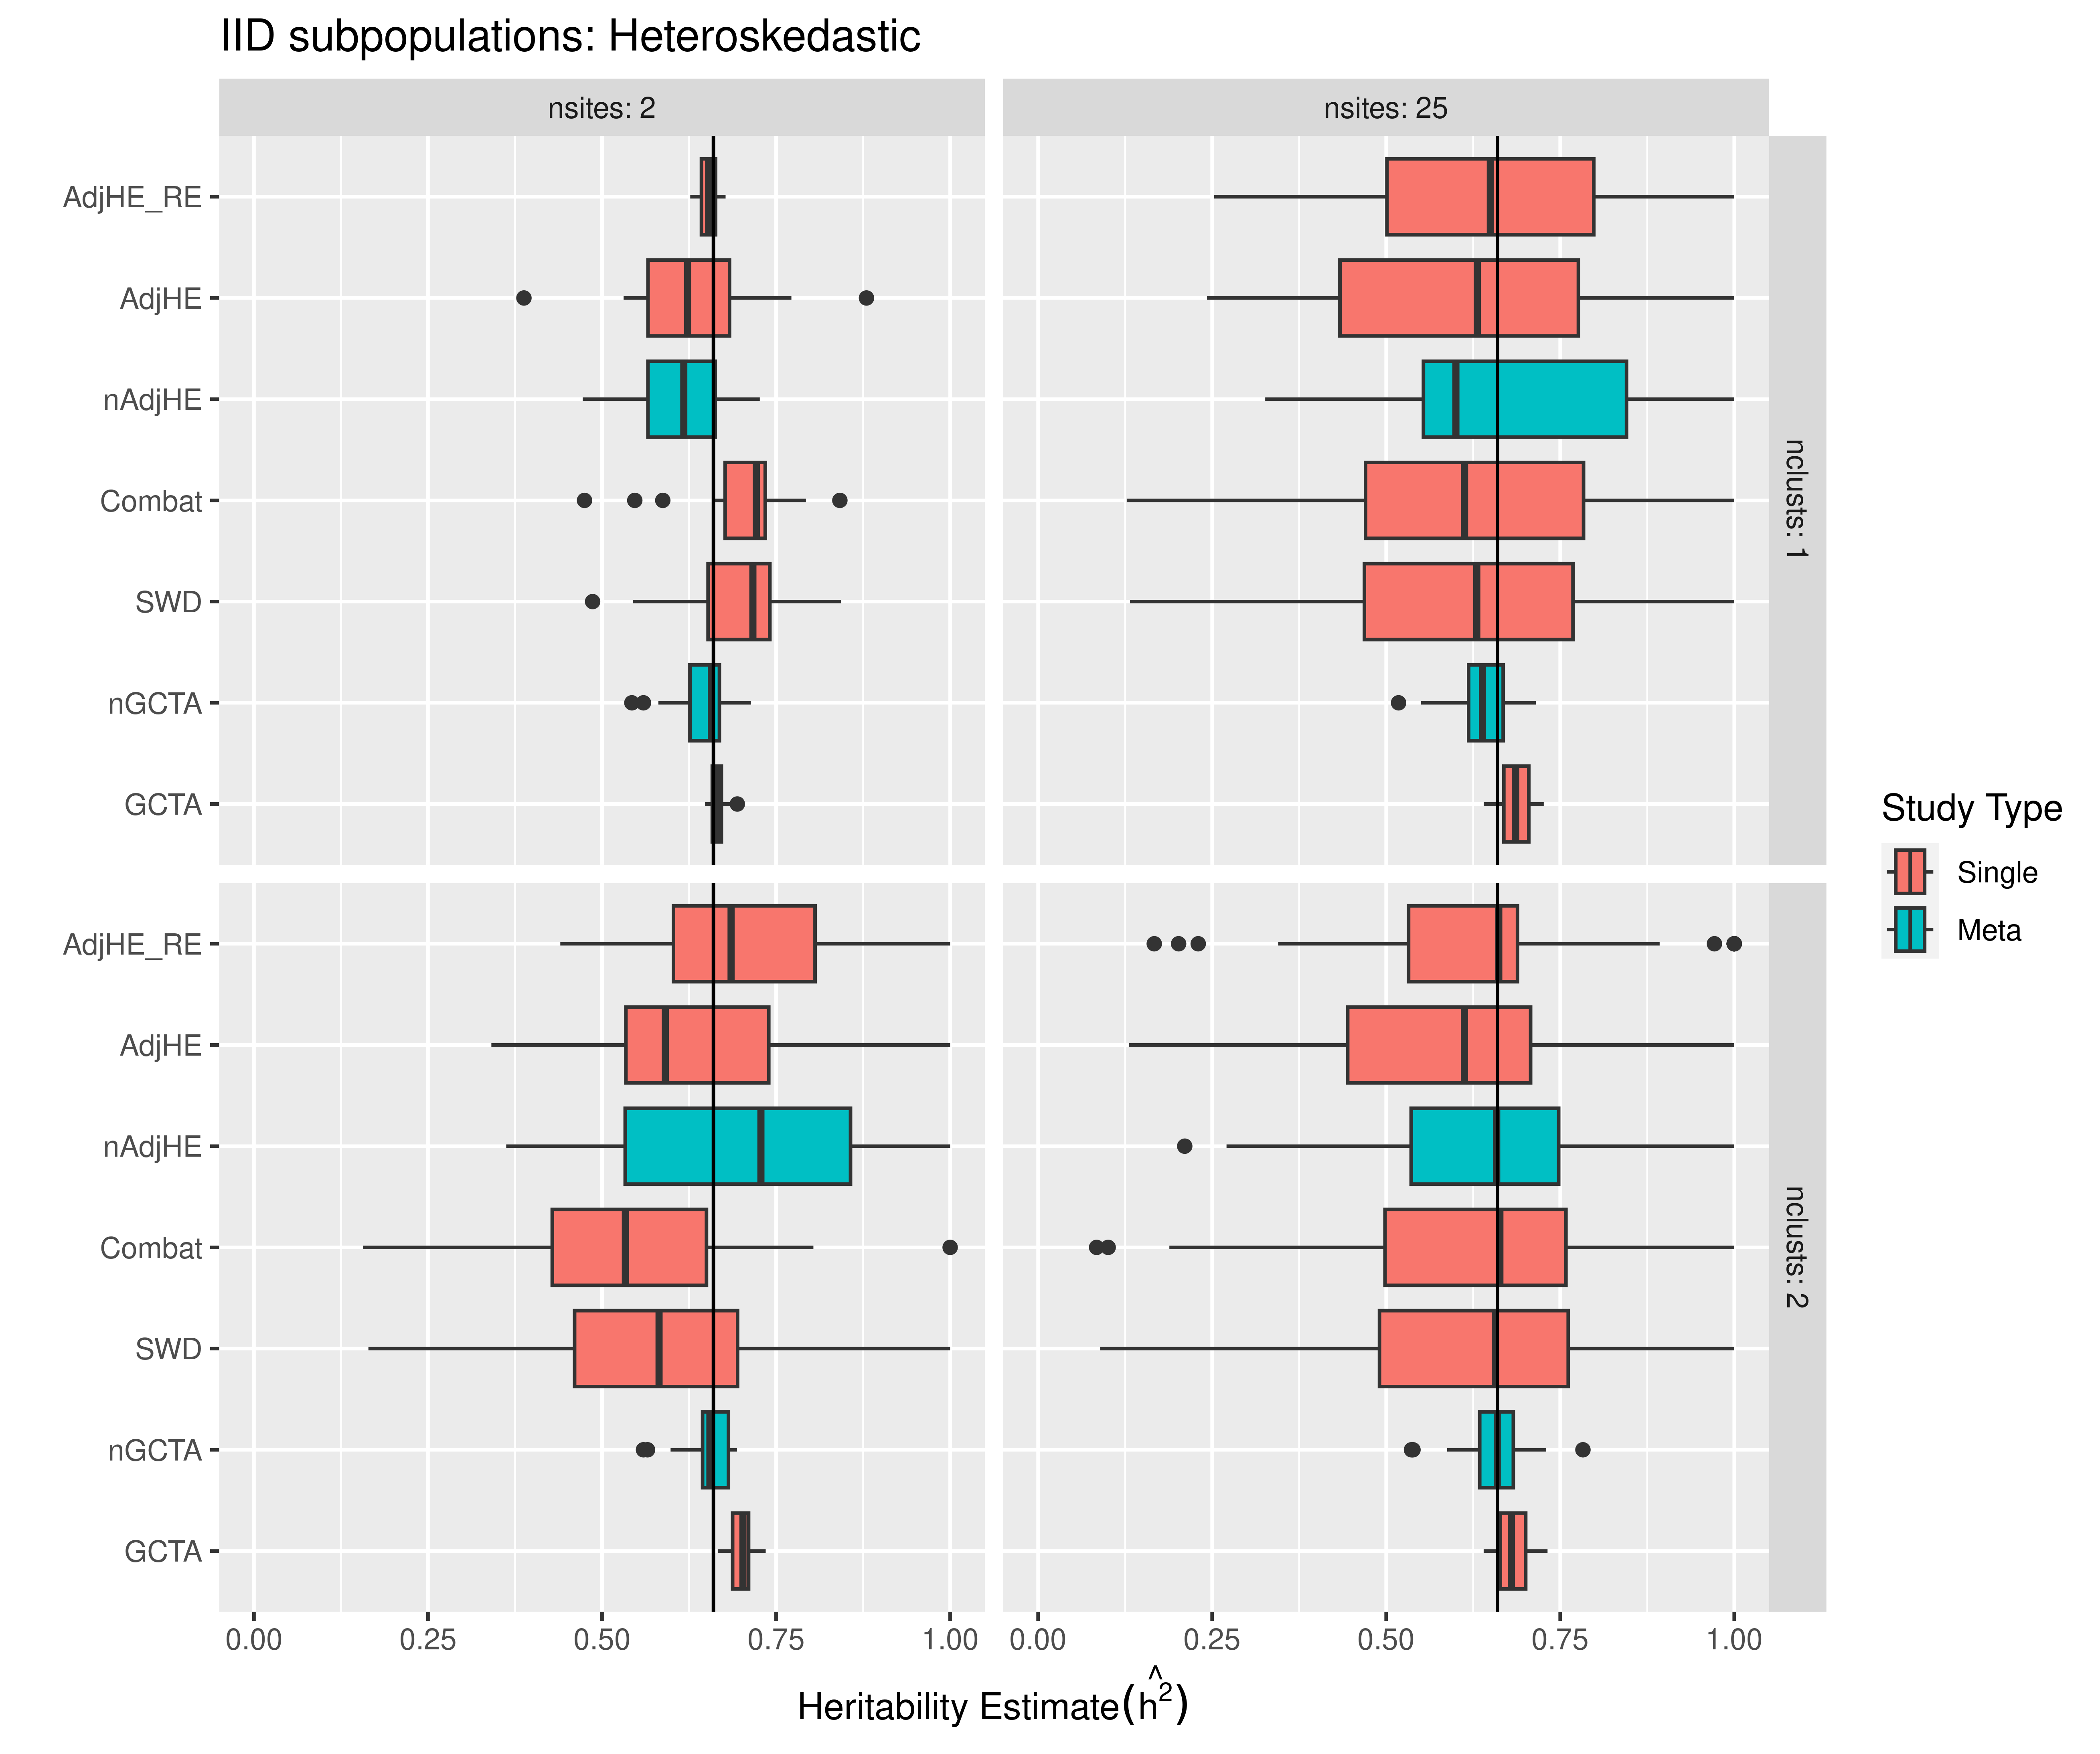
\includegraphics[width=0.66\textwidth]{Graphics/Adding_sites_n_clusts_het.png}
    \caption{\centering
       Simulation estimates under 2 and 25 sites (left and right columns) and 1 and 2 genetic ancestries (top and bottom rows). Estimates are compared between the proposed method "AdjHE\_RE" and multiple other methods including GCTA.
    } \label{fig:03-03}
\end{figure}

\begin{alertblock}{Contact}
Email: coffm049@umn.edu \\
Github: https://github.com/coffm049
\end{alertblock}


\end{column} % End of the second column
\begin{column}{\sepwid}\end{column} % Empty spacer column
\begin{column}{\onecolwid} % The third column
%----------------------------------------------------------------------------
%	RIGHT
%----------------------------------------------------------------------------
\begin{block}{Discussion}
The new estimator broadens unbiased estimation to conditions where genetic ancestries and site effects vary between sites. We've shown the new estimator is unbiasedness theoretically and through simulations. In addition, we found multiple regions with significant heritability in the adolescent brain. We next hope to extend this method to multivariate traits.
\end{block}

\vspace{3cm}

\begin{block}{ABCD Demographics}
\begin{figure}
    \centering
    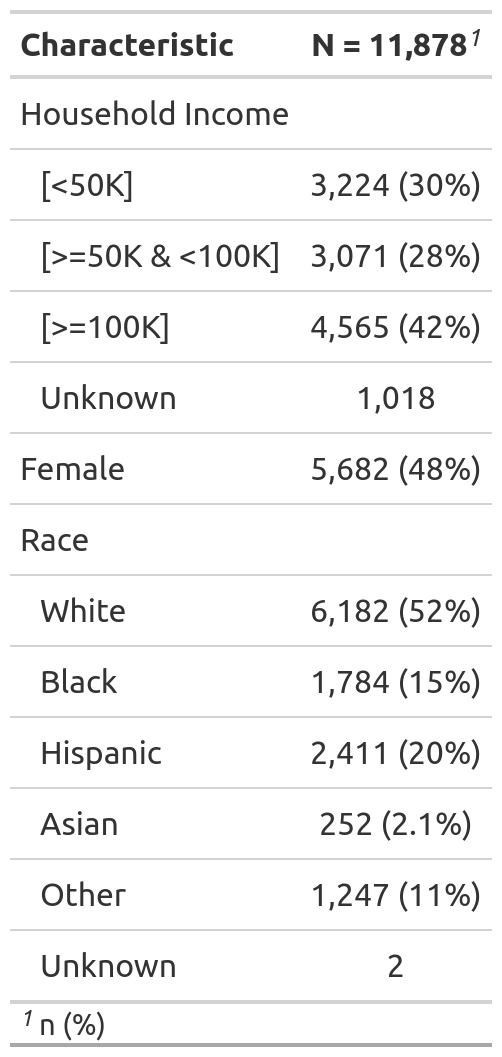
\includegraphics[width = 1\textwidth]{Graphics/Table1.png}
    \caption{Descriptions of key demographic variables in the ABCD dataset.
}
    \label{tab:table}
\end{figure}
\end{block}



%----------------------------------------------------------------------------
%	REFERENCES
%----------------------------------------------------------------------------
\begin{block}{References}
	\begin{tiny}
		\bibliographystyle{abbrv}
		\bibliography{Mycoll}
	\end{tiny}
\end{block}

%----------------------------------------------------------------------------
%	ACKNOWLEDGEMENTS
%----------------------------------------------------------------------------
\begin{block}{Acknowledgements}
This research was funded through an NIH T32 grant (GM132063).
\end{block}

%----------------------------------------------------------------------------
%----------------------------------------------------------------------------


%----------------------------------------------------------------------------
\end{column} % End of the third column
\end{columns} % End of all the columns in the poster
\end{frame} % End of the enclosing frame
\end{document}


